\documentclass[oneside,11pt,a4paper]{article}

% Chargement d'extensions
\usepackage[utf8]{inputenc}
\usepackage[french]{babel}
\usepackage{graphicx}
\usepackage[top=3cm, bottom=3cm, left=3cm, right=3cm]{geometry}
\usepackage{amsmath}
\usepackage{amssymb}

% Bout de code
\usepackage{listings}
\usepackage{color}

\definecolor{mygreen}{rgb}{0,0.6,0}
\definecolor{mygray}{rgb}{0.5,0.5,0.5}
\definecolor{mymauve}{rgb}{0.58,0,0.82}

% Commande pour notation 'NB :' (nota bene)
\newcommand\nb[1][0.3]{N\kern-#1emB : }

% csquotes va utiliser la langue définie dans babel
\usepackage[babel=true]{csquotes}

% pour afficher Schéma au lieu de figure dans les legende des images
\addto\captionsfrench{\def\figurename{Schéma}}

% Informations le titre, le(s) auteur(s), la date
\title{Evarois}
\author{
    Ramzi ZEROUAL \and
    Belkassim BOUZIDI
}
\date{\today}


\begin{document}
%\maketitle
\begin{titlepage}
	\centering
	{\scshape\LARGE Universite de Montpellier\par}
	{\scshape\Large Rapport de projet web\par}
	\vspace{1.5cm}
	{\huge\bfseries  Evarois \par}
	\vspace{2cm}
	\begin{figure}[h]
		\centering
		
\includegraphics[width=0.4\textwidth]{logo.jpg}
	\end{figure}
	\vspace{2cm}
	{\Large\itshape
	Ramzi ZEROUAL \\
    Belkassim BOUZIDI \\
		\par}

	\vspace{1.5cm}


	
\vfill
	% Bottom of the page
	{\large \today\par}
\end{titlepage}
\section{Introduction}

Le travail présenté dans le cadre d'un projet web pour le module  HLIN510 - Architecture et programmation du web  , est de créer un site web spécialisée dans les expériences partagées qui permet à chaque habitant de la région var provance côté dazure de créer, partager, trouver et participer à des événements .

\section{Modélisation}

Tout d'abord nous avons modélisé notre base de données de la manière suivante : 

\begin{figure}[h]
  \centering
  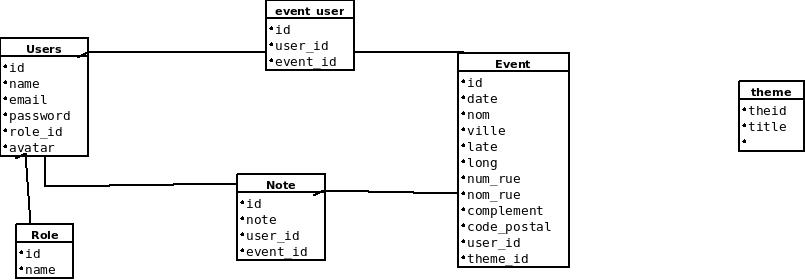
\includegraphics[width=1\textwidth]{Diagramme1.jpg}
  \caption{Modèl E/A}
\end{figure}
  
\section{Technologies utilisées}

Pour ce projet nous avons décidé d'en profiter et apprendre un framework qui est Laravel , Laravel est un framework web open-source écrit en PHP respectant le principe modèle-vue-contrôleur et entièrement développé en programmation orientée

Puis pour mieux structurer les differents fichiers sources nous avons decidé d'utiliser la structure MVC (pour Model View Controller). Nous avons donc stocker tout nos fichiers dans trois dossiers : Model, View et Controller. Les fichiers du model se charge d'intéragir avec la base de données, les fichiers dans le dossier view se charge d'afficher et de donnez du style à nos pages, enfin les fichiers du dossier Controller fait la liason entre le model et les View. (voir : https://fr.wikipedia.org/wiki/Mod\%C3\%A8le-vue-contr\%C3\%B4leur).
\section{Foncionnalitées implementées}

Sur toutes les foncionnalitées demandées, nous les avons toutes implementées sauf :

\begin{itemize}
  \item La visualisation des événements sur une carte , le problème ici a été d'afficher la map où l'évenement est situé , la fonction php qui permet de récuperer " lat " et "long" est fonctionnel , l'érreur se trouve surement dans le script js.

  \item L'ajout de photos pour un évenement , cette foncionnalitée marchais normalment quelques jours avant d'avoir rendu le projet.
\end{itemize}

\begin{itemize}
\item Par contre, nous avons implementé la possibilité pour un utilisateur, une fois inscrit, de visualiser les évenements aux quelles il a participé et ceux aux quelles il participera.

\end{itemize}
\section{Conclusion}

\subsection{Les problèmes recontrés}
\begin{itemize}
\item Lors du développement du projet, nous avons du recommencer le projet à cause d'un problème sur GitHub.
\item Le déploiement du site a été aussi un problème , nous n'avons pas réussi a déployer le site correctement
\end{itemize}


\subsection{Les compètences acquises}

Pour conclure, à l’issue de ce projet nous avons réussi à réaliser un site web fonctionnel et prèt à l'utilisation. 

Ce projet nous aura permis d’aprofondir nos connaissances en développement web et de compléter nos acquis sur les outils de base du web, tel que :HTML, CSS, PHP et JAVASCRIPT.

\end{document}